%%%%%%%%%%%%%%%%%%%%%%%%%%%%%%%%%%%%%%%%%
% Stylish Article
% LaTeX Template
% Version 2.2 (2020-10-22)
%
% This template has been downloaded from:
% http://www.LaTeXTemplates.com
%
% Original author:
% Mathias Legrand (legrand.mathias@gmail.com) 
% With extensive modifications by:
% Vel (vel@latextemplates.com)
%
% License:
% CC BY-NC-SA 3.0 (http://creativecommons.org/licenses/by-nc-sa/3.0/)
%
%%%%%%%%%%%%%%%%%%%%%%%%%%%%%%%%%%%%%%%%%

% SNIPPET UTILI %


%----------------------------------------------------------------------------------------
%	PACKAGES AND OTHER DOCUMENT CONFIGURATIONS
%----------------------------------------------------------------------------------------

\documentclass[fleqn,10pt]{SelfArx} % Document font size and equations flushed left

%\usepackage[english]{babel} % Specify a different language here - english by default
\usepackage[italian]{babel} % Specify a different language here - english by default

\usepackage{lipsum} % Required to insert dummy text. To be removed otherwise

%----------------------------------------------------------------------------------------
%	COLUMNS
%----------------------------------------------------------------------------------------

\setlength{\columnsep}{0.55cm} % Distance between the two columns of text
\setlength{\fboxrule}{0.75pt} % Width of the border around the abstract

%----------------------------------------------------------------------------------------
%	COLORS
%----------------------------------------------------------------------------------------

\definecolor{color1}{RGB}{0,0,90} % Color of the article title and sections
\definecolor{color2}{RGB}{0,20,20} % Color of the boxes behind the abstract and headings

%----------------------------------------------------------------------------------------
%	HYPERLINKS
%----------------------------------------------------------------------------------------

\usepackage{hyperref} % Required for hyperlinks

\hypersetup{
	hidelinks,
	colorlinks,
	breaklinks=true,
	urlcolor=color2,
	citecolor=color1,
	linkcolor=color1,
	bookmarksopen=false,
	pdftitle={Title},
	pdfauthor={Author},
}

%----------------------------------------------------------------------------------------
%	ARTICLE INFORMATION
%----------------------------------------------------------------------------------------

\JournalInfo{Programmazione per l'IoT - Laurea Magistrale in Informatica Applicata - DiSPeA - Università degli Studi di Urbino Carlo Bo} % Journal information
\Archive{Data di pubblicazione xx/xx/xxxx - DOI: xxxx/xxxxxxx} % Informazioni che verranno inserite dal Docente in fase di pubblicazione

\PaperTitle{4.0 Gym Prototype} % Article title

\Authors{Luca Cinti\textsuperscript{1}*, Emanuele Lattanzi\textsuperscript{2}} % Il docente Emanuele Lattanzi figura come autore
% al fine di poter gestire la procedura di submission sul repository pubblico (nell'affiliazione viene chiarito il ruolo)
\affiliation{\textsuperscript{1}\textit{Laurea Magistrale in Informatica Applicata, Università degli Studi di Urbino Carlo Bo, Urbino, Italia}} % Author affiliation
\affiliation{\textsuperscript{2}\textit{Docente di Programmazione per l'Internet of Things, Università degli Studi di Urbino Carlo Bo, Urbino, Italia}} % Author affiliation
\affiliation{*\textbf{Corresponding author}: l.cinti@campus.uniurb.it} % Corresponding author

\Keywords{IOT --- Arduino --- ESP32 --- MQTT --- Gym Metrics} % Keywords - if you don't want any simply remove all the text between the curly brackets
\newcommand{\keywordname}{Keywords} % Defines the keywords heading name

%----------------------------------------------------------------------------------------
%	ABSTRACT
%----------------------------------------------------------------------------------------

\Abstract{
	In questo elaborato abbiamo cercato di predisporre un'architettura per la raccolta dei dati
	in una piccola home gym, innanzitutto per verificare la fattibilità nel reperimento di alcune misurazioni, 
	per poi passare all'analisi dei dati raccolti, con l'obiettivo di estrapolare delle metriche significative 
	sia ai fini dell'allenamento, che dello studio delle caratteristiche termiche dell'ambiente.
}

%----------------------------------------------------------------------------------------

\begin{document}

\maketitle % Output the title and abstract box

%\tableofcontents % Output the contents section

\thispagestyle{empty} % Removes page numbering from the first page

%----------------------------------------------------------------------------------------
%	ARTICLE CONTENTS
%----------------------------------------------------------------------------------------

\section*{Introduzione} % The \section*{} command stops section numbering
%\lipsum[1-3] % Dummy text
% and some mathematics $\cos\pi=-1$ and $\alpha$ in the text\footnote{And some mathematics $\cos\pi=-1$ and $\alpha$ in the text.}
%Questa è una citazione al libro di testo~\cite{milenkovic2020internet}.

% \begin{enumerate}[noitemsep] % [noitemsep] removes whitespace between the items for a compact look
% 	\item First item in a list
% 	\item Second item in a list
% 	\item Third item in a list
% \end{enumerate}

% \begin{equation}
% 	\cos^3 \theta =\frac{1}{4}\cos\theta+\frac{3}{4}\cos 3\theta
% 	\label{eq:refname2}
% \end{equation}

% \subsection{Subsection}

% \paragraph{Paragraph} \lipsum[7] % Dummy text
% \paragraph{Paragraph} \lipsum[8] % Dummy text

% \subsection{Subsection}

% \lipsum[9] % Dummy text

% Reference to Figure \ref{fig:results}.

% \begin{figure}[ht]\centering
% 	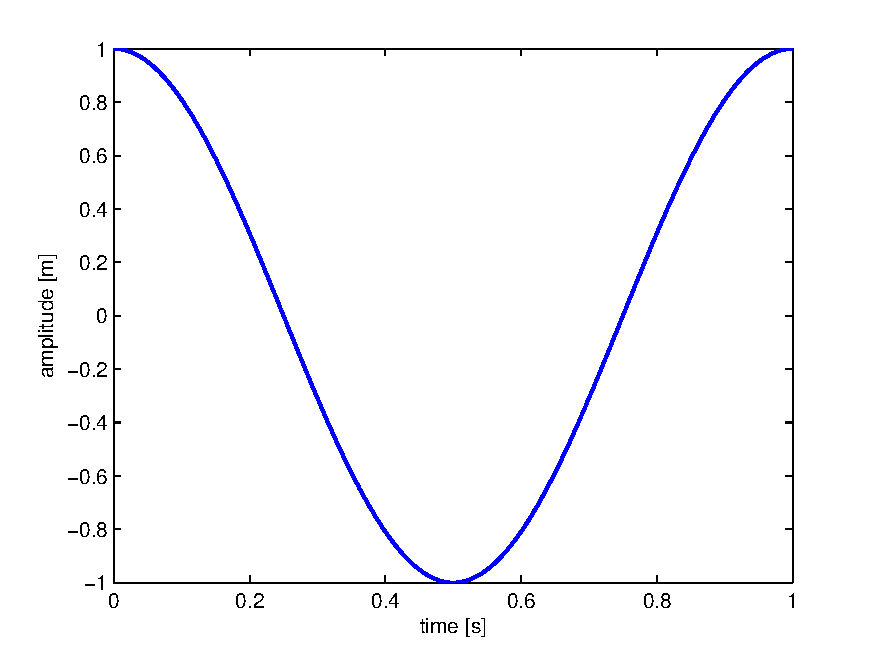
\includegraphics[width=\linewidth]{results}
% 	\caption{In-text Picture}
% 	\label{fig:results}
% \end{figure}

% \begin{description}
% 	\item[Word] Definition
% 	\item[Concept] Explanation
% 	\item[Idea] Text
% \end{description}

L'obiettivo preliminare di questo elaborato era verificare la fattibilità dell'allestimento di un sistema di 
raccolta dati, in una piccola home gym, costruendo l'infrastruttura per far comunicare 
attraverso diversi protocolli una rete di sensori.\\

Tra le più disparate metriche di possibile interesse ai fini dello studio di una palestra, 
sono state scelte due categorie di dati: da un lato i quelli relativi all'ambiente di allenamento, 
dall'altro i dati sull'esecuzione degli esercizi.

Per il progetto corrente sono state dunque prese in analisi le metriche seguenti:

\begin{itemize}[noitemsep] % [noitemsep] removes whitespace between the items for a compact look
	\item temperatura e umidità della stanza, prima durante e dopo l'allenamento
	\item variazione di CO\textsubscript{2} e TVOC (Total Volatile Organic Compounds)
	\item accelerazione del bilanciere durante l'esecuzione di un esercizio campione
\end{itemize}

\section{Descrizione dell'ambiente}

Funzionale alla comprensione di questo elaborato, è la descrizione dell'ambiente in cui è stata allestita 
la palestra: si tratta di una stanza appartenente ad un vecchio immobile disabitato, appositamente 
ristrutturata, le cui misure sono 5.05 x 4.95 metri, per un'altezza di 3.86 metri. \\

L'ambiente presenta una finestra, una porta finestra e un'arcata di ingresso sulla quale sono state applicate 
due tende, fissate con velcro ai lati del muro, come isolante dal resto del locale, in quanto non 
sono presenti sistemi di riscaldamento centralizzato. Possiamo vederne una panoramica nell'immagine che segue 
(Figura 2). \\

Il primo punto di analisi è dunque diretta conseguenza di quanto appena detto: analizzare le performance 
termiche dell'ambiente, per trovare il miglior metodo di riscaldamento durante i mesi invernali.\\
Collegato a questo vi è il secondo punto in analisi: riscaldando un ambiente di circa 96 metri cubici, quanto 
più possibile isolato dal resto del locale, abbiamo ritenuto importante monitorare la qualità dell'aria 
durante l'allenamento.

\section{Scelta della terza metrica}
Come abbiamo visto in precedenza, come terzo oggetto di studio è stata presa in analisi l'accelerazione del bilanciere 
durante l'esecuzione di un esercizio campione.\\
L'esercizio selezionato è la distensione su panca piana, scelto in quanto ci garantiva il maggior grado di controllo 
sull'esecuzione, essendo uno degli esercizi base di ogni allenamento. Ne possiamo vedere uno schema in Figura 1.\\

La popolarità di tale esercizio ci garantiva inoltre buone potenzialità di espansione di questo studio, ad un 
ampio campione di tester, nel caso fossimo riusciti a standardizzare il più possibile il metodo di acquisizione dei dati.

\begin{figure}[htb!]\centering
	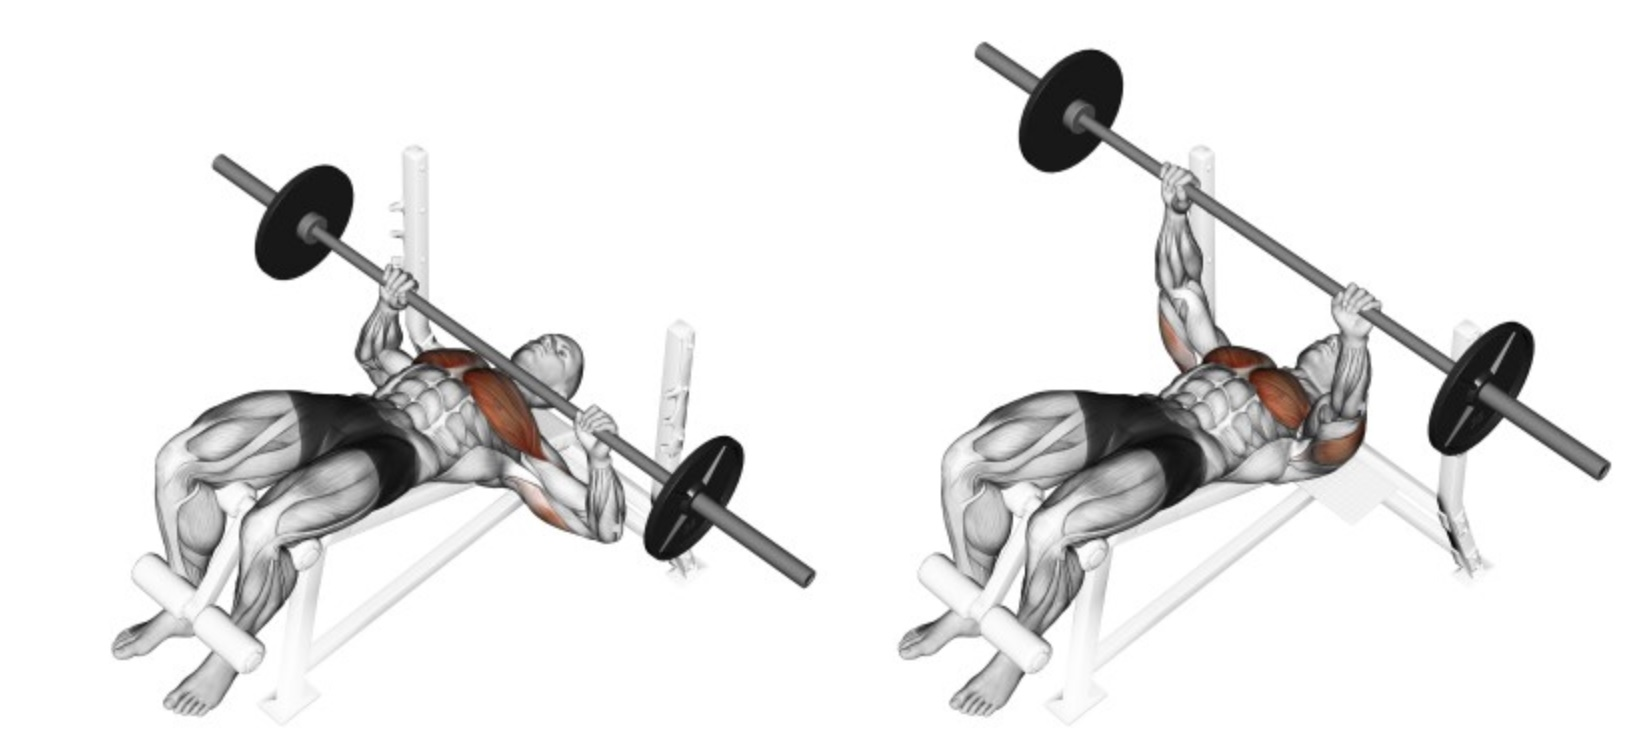
\includegraphics[width=\linewidth]{panca_piana}
	\caption{distensioni su panca piana}
	\label{fig:panca_piana}
\end{figure}

\begin{figure*}[ht]\centering % Using \begin{figure*} makes the figure take up the entire width of the page
	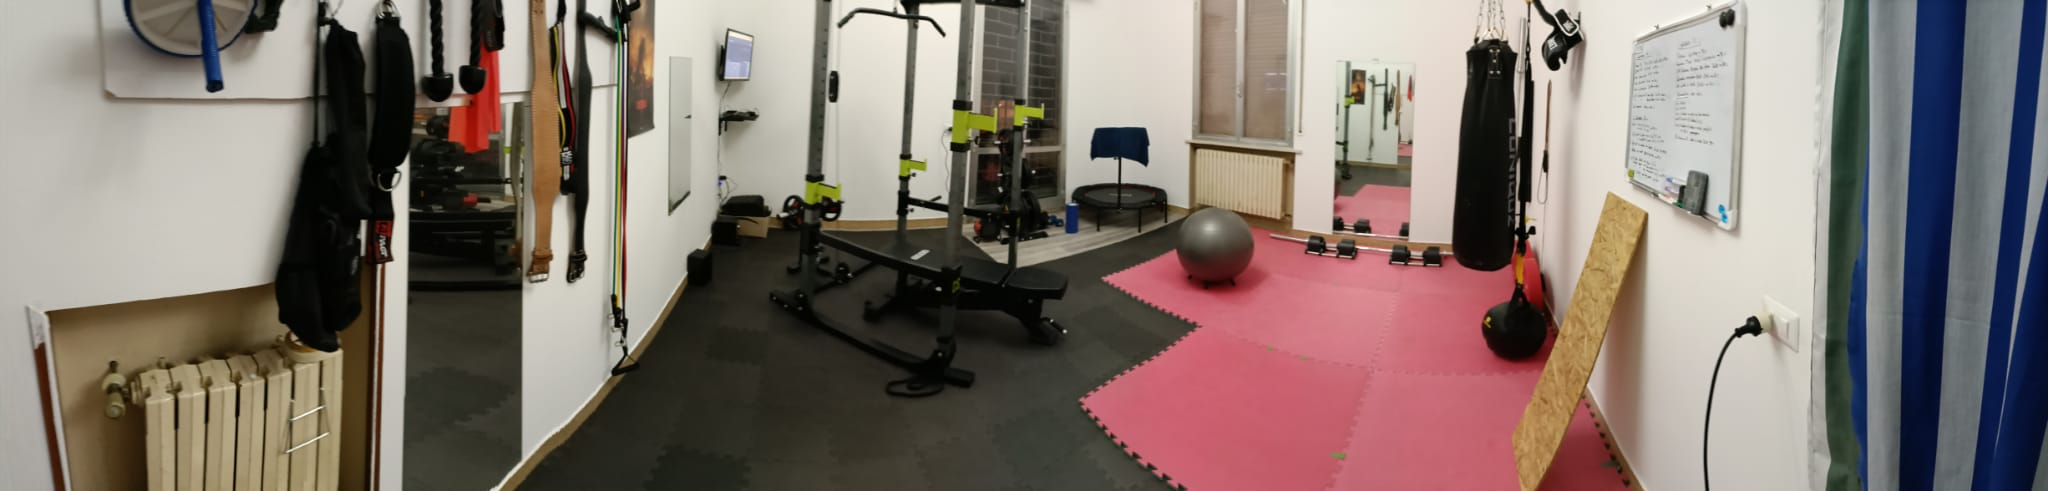
\includegraphics[width=\linewidth]{panoramica_palestra}
	\caption{Visione panoramica dell'ambiente}
	\label{fig:view}
\end{figure*}

%------------------------------------------------

\section{Allestimento dell'infrastruttura}

La prima necessità è stata dunque quella di creare l'infrastruttura attraverso la quale sarebbe avvenuta la 
comunicazione dei dati.\\
A livello di rete e internet sono stati fatti diversi tentativi, prima con due diversi router extender che 
prolungavano una casalinga fino al locale della palestra, e poi con un router con scheda SIM 
situato direttamente in loco. La prima soluzione è stata scartata in quanto, ad una distanza in linea d'aria 
dal router di casa di circa cinquanta metri, senza considerare i muri, la connessione era troppo instabile.\\

A questa rete è stato poi collegato un Raspberry Pi 4 che ha fatto sia da broker MQTT (di cui parleremo in seguito), 
che da semplice computer per la raccolta e visualizzazione dei dati, come vediamo in Figura 3.

\begin{figure}[htb!]\centering
	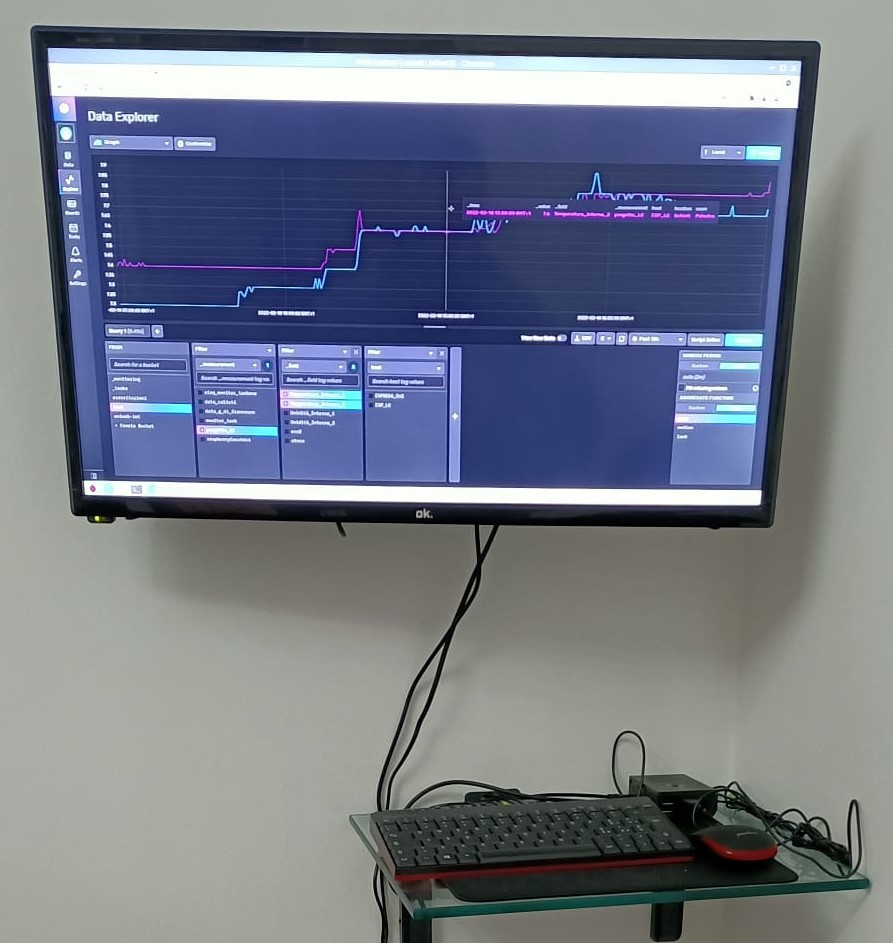
\includegraphics[width=\linewidth]{schermo_dati}
	\caption{Raspberry e monitor}
	\label{fig:schermo}
\end{figure}

\subsection{I sensori utilizzati}

Per raccogliere i dati sono stati utilizzati i seguenti sensori:

\begin{itemize}[noitemsep] % [noitemsep] removes whitespace between the items for a compact look
	\item due DHT11 per temperatura e umidità
	\item due DHT22 per temperatura e umidità
	\item un CCS811 per CO\textsubscript{2} e TVOC
	\item due GY-521 MPU-6050 per l'accelerazione
\end{itemize}

Si è scelto di collegare gli accelerometri a dei moduli di sviluppo ESP32 mini, potendo così accedere ad 
un'architettura double core, mentre tutti gli altri sensori sono stati collegati a delle normali ESP8266. 
Abbiamo adottato sensori DHT11 e DHT22 per temperatura e umidità, potendo così avere un confronto nella 
precisione dei due: vediamo le differenze tra le loro specifiche nella tabella che segue.

\begin{table}[hbt]
	\caption{Specifiche DHT}
	\centering
	\begin{tabular}{lcc}
		\toprule
			 & \textbf{DHT11} & \textbf{DHT22} \\
		\midrule
		Range umidità & 20-90\% & 0-100\% \\
		Precisione umidità & ±5\% & ±2\% \\
		Range temperatura & 0-50 °C & -40 +80 °C \\
		Precisione temperatura & ±2\% & ±0.5\% \\
		Tempo di lettura & 6-10 s & 2 s \\
		\bottomrule
	\end{tabular}
	\label{tab:label}
\end{table}

Nelle tre immagini che seguono (Figure 4, 5, 6) sono mostrati gli schemi dei circuiti costruiti: 

\begin{figure}[htb!]\centering
	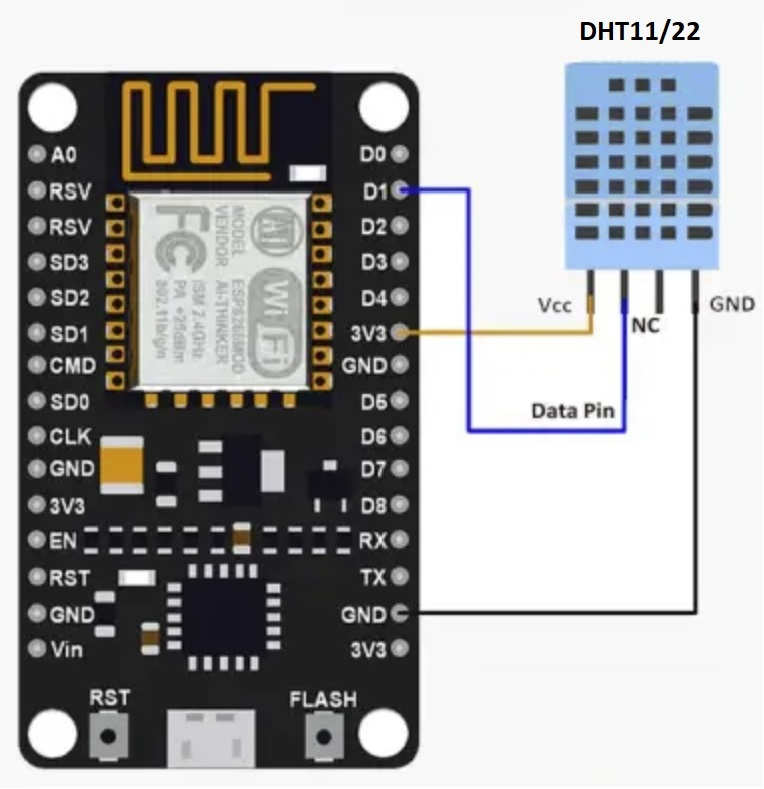
\includegraphics[scale=0.5]{DHT}
	\caption{ESP8266 - DHT11/22}
	\label{fig:schermo}
\end{figure}

\begin{figure}[htb!]\centering
	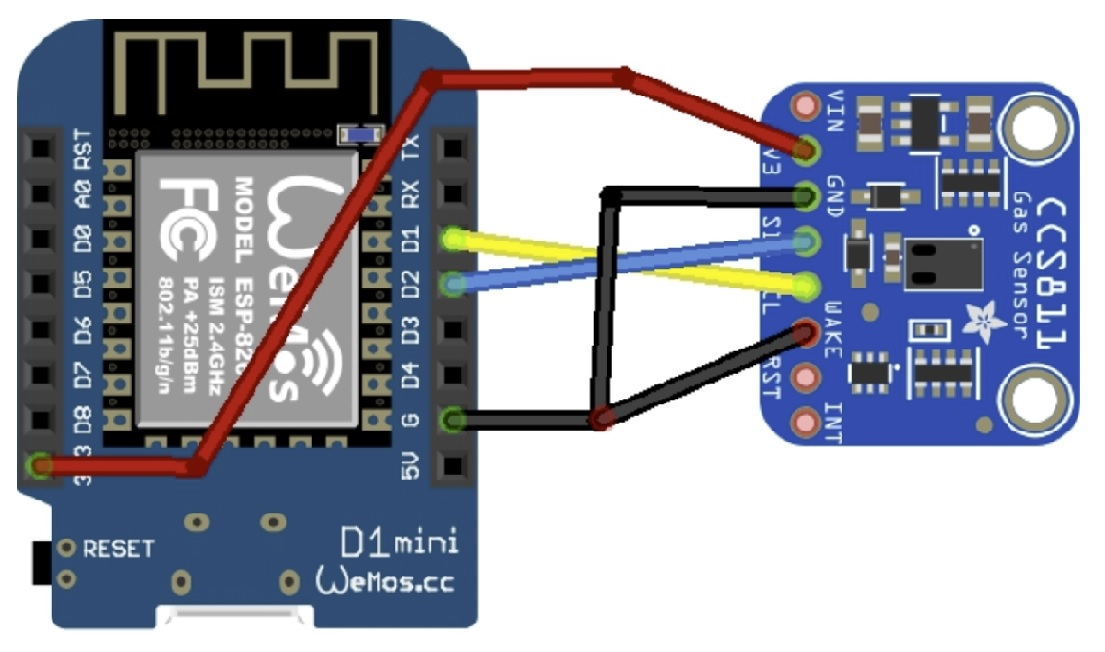
\includegraphics[scale=0.5]{CCS811}
	\caption{ESP8266 - CCS811}
	\label{fig:schermo}
\end{figure}

\begin{figure}[htb!]\centering
	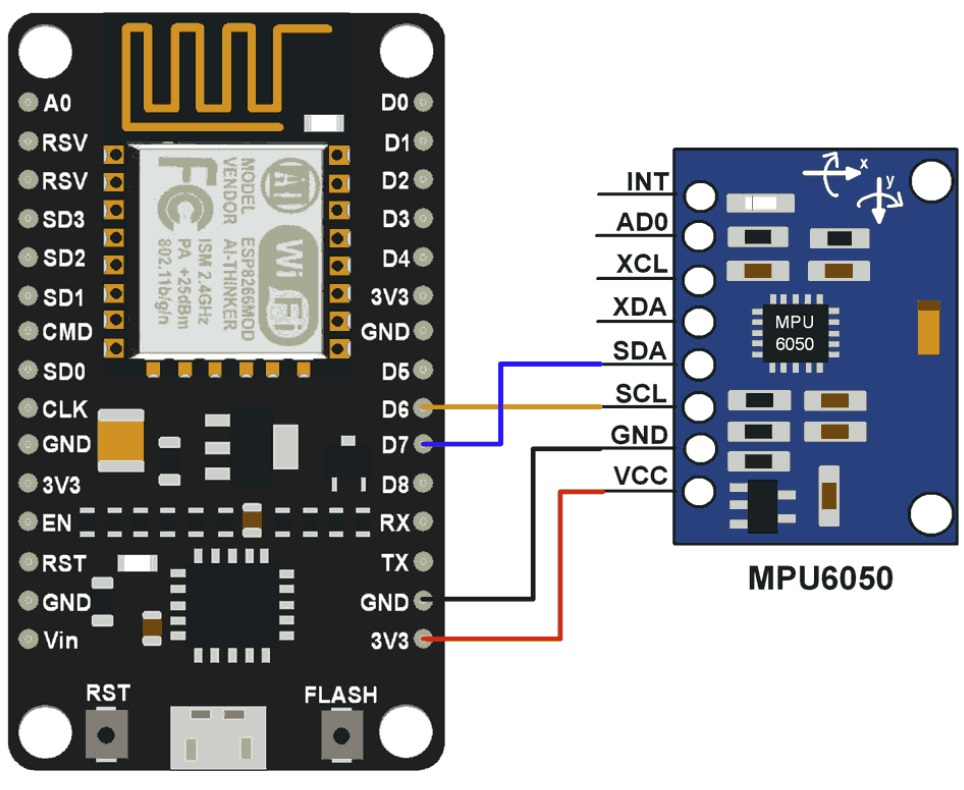
\includegraphics[scale=0.5]{Schema_accelerometro}
	\caption{ESP32 - MPU-6050}
	\label{fig:schermo}
\end{figure}

Per motivi che vedremo in seguito, due postazioni di rilevamento della temperatura e dell'umidità sono state 
implementate con batteria e un meccanismo di deep sleep per il risparmio energetico, nei relativi circuiti erano 
dunque presenti i collegamenti per una batteria da 650 mA e un jumper per consentire la programmazione del modulo.

\subsubsection{Gli accelerometri e i loro obiettivi}

Un discorso a parte va fatto per gli accelerometri, che costituiscono la parte principale di questo studio.\\
Innanzitutto è necessario chiarire l'obiettivo dell'analisi, ovvero cercare di registrare 
se, nell'esecuzione di un qualsiasi esercizio che coinvolga il sollevamento di un bilanciere, si rilevano delle 
imperfezioni, da cogliere attraverso le differenze nelle accelerazioni agli estremi dell'attrezzo: se un accelerometro 
posto a un estremo del bilanciere, avesse riscontrato accelerazioni diverse da quelle registrate 
all'estremo opposto, sarebbe stato possibile individuare delle imperfezioni nell'esecuzione dell'esercizio, 
dandoci così un feedback sulla qualità dello stesso, ed eventuali indicazioni per migliorarlo.\\

Con questo obiettivo in mente abbiamo ritenuto imprescindibile che entrambi i moduli fossero alimentati a batteria, 
per evitare perturbazioni nelle misurazioni dovute ad eventuali interferenze dei fili di alimentazione. Questo ha però 
aumentato la difficoltà nella costruzione del "sistema accelerometro", che includendo ora anche una batteria, 
diventava più ingombrante e difficilmente stabilizzabile sul bilanciere.\\

La soluzione che abbiamo adottato è stata quella di costruire delle piccole scatole di plastica, appositamente 
progettate in base alle misure del modulo ESP32 mini col sensore e la batteria. Queste scatole sono state poi fissate 
agli anelli di bloccaggio dei dischi al bilanciere. Ne possiamo vedere il risultato nella Figura 7.


\section{Risultati}

\subsection{Subsection}


\subsubsection{Subsubsection}

\subsubsection{Subsubsection}

\section{Conclusioni}

%----------------------------------------------------------------------------------------
%	REFERENCE LIST
%----------------------------------------------------------------------------------------

\phantomsection
\bibliographystyle{unsrt}
\bibliography{sample.bib}

%----------------------------------------------------------------------------------------

\end{document}